\documentclass[11pt,a4paper]{article}
\usepackage[utf8]{inputenc}
\usepackage[T1]{fontenc}
\usepackage{amsthm} %numéroter les questions
\usepackage[frenchb]{babel}
\usepackage{datetime}
\usepackage{xspace} % typographie IN
\usepackage{hyperref}% hyperliens
\usepackage[all]{hypcap} %lien pointe en haut des figures
\usepackage[french]{varioref} %voir x p y
\usepackage{fancyhdr}% en têtes
%\input cyracc.def
\usepackage[]{graphicx} %include pictures
\usepackage{pgfplots}
\usepackage[]{circuitikz}
\usepackage{ifthen}

\usepackage[top=1.3 in, bottom=1.3 in, left=1.3 in, right=1.3 in]{geometry} % Yeah, that's bad to play with margins
\usepackage[]{pdfpages}

\usepackage[]{attachfile}

\usepackage{float}
\usepackage{subfig}

\usepackage{todonotes} % \missingfigure
\usepackage{gensymb} % \ohm

\usepackage{framed}

\newdateformat{mydate}{2016--2017}%hack pour remplacer \THEYEAR


\newboolean{corrige}
\ifx\correction\undefined
\setboolean{corrige}{false}% pas de corrigé
\else
\setboolean{corrige}{true}%corrigé
\fi

%\setboolean{corrige}{false}% pas de corrigé

\newboolean{annexes}
\setboolean{annexes}{true}%annexes
%\setboolean{annexes}{false}% pas de annexes

\definecolor{darkblue}{rgb}{0,0,0.5}

\newboolean{mos}
%\setboolean{mos}{true}%annexes
\setboolean{mos}{false}% pas de annexes

\usepackage{aeguill} %guillemets

%% fancy header & foot
\pagestyle{fancy}
%Numero du TP :
\def \labonumber {Projet -- Partie 1}
\lhead{[ELEC-H-310] Choucroute numérique\\ \labonumber}
\rhead{\mydate\today\\ page \thepage}
\chead{\ifthenelse{\boolean{corrige}}{Corrigé}{}}
\cfoot{}
%%

\pdfinfo{
/Author (Quentin Delhaye, Ken Hasselmann, ULB -- BEAMS)
/Title (\labonumber ELEC-H-310)
/ModDate (D:\pdfdate)
}

\hypersetup{
pdftitle={\labonumber [ELEC-H-310] Choucroute numérique},
pdfauthor={Quentin Delhaye, Ken Hasselmann, ULB -- BEAMS},
pdfsubject={}
}

\theoremstyle{definition}% questions pas en italique
\newtheorem{Q}{Question}[] % numéroter les questions [section] ou non []

\newcommand{\reponse}[1]{% pour intégrer une réponse : \reponse{texte} : sera inclus si \boolean{corrige}
	\ifthenelse {\boolean{corrige}} {\paragraph{Réponse :} \color{darkblue}   #1\color{black}} {}
 }

\newcommand{\addcontentslinenono}[4]{\addtocontents{#1}{\protect\contentsline{#2}{#3}{#4}{}}}

\date{\vspace{-1.7cm}\mydate\today}
\title{\vspace{-2cm}\labonumber \\ Électronique numérique [ELEC-H-310]\\Conception d'une régulation de refroidissement~: \\ pré-étude et alimentation de l'hélice\ifthenelse{\boolean{corrige}}{~\\Corrigé}{}}

%\author{\vspace{-1cm}}%\textsc{Yannick Allard}}

\setlength{\parskip}{0.2cm plus2mm minus1mm} %espacement entre §
\setlength{\parindent}{0pt}






%%%%%%%%%%%%%%%%%%%%%%%%%%%%%%%%%%%%%%%%%%%%%%%%%%%%%%%%%%%%%%%%%%%%%%%%%%%%%%%%%%%%%%%%%%%%%%%%%%%%%%%%%%%%%
%%%%%%%%%%%%%%%%%%%%%%%%%%%%%%%%%%%%%%%%%%%%%%%%%%%%%%%%%%%%%%%%%%%%%%%%%%%%%%%%%%%%%%%%%%%%%%%%%%%%%%%%%%%%%
%%%%%%%%%%%%%%%%%%%%%%%%%%%%%%%%%%%%%%%%%%%%%%%%%%%%%%%%%%%%%%%%%%%%%%%%%%%%%%%%%%%%%%%%%%%%%%%%%%%%%%%%%%%%%
% http://tex.stackexchange.com/questions/128123/circuitikz-current-source
% preparation to create bipoles

\makeatletter
\def\TikzBipolePath#1#2{\pgf@circ@bipole@path{#1}{#2}}

\pgf@circ@Rlen = \pgfkeysvalueof{/tikz/circuitikz/bipoles/length}
\makeatother 

\newlength{\ResUp} \newlength{\ResDown}
\newlength{\ResLeft} \newlength{\ResRight}

% set default dohicky size

\ctikzset{bipoles/doohicky/height/.initial=.4}
\ctikzset{bipoles/doohicky/width/.initial=.6}

% create doohicky shape

\pgfcircdeclarebipole{}
 {\ctikzvalof{bipoles/doohicky/height}}
 {doohicky}
 {\ctikzvalof{bipoles/doohicky/height}}
 {\ctikzvalof{bipoles/doohicky/width}}
 {
    \pgfsetlinewidth{\pgfkeysvalueof{/tikz/circuitikz/bipoles/thickness}\pgfstartlinewidth}
    \pgfextractx{\ResRight}{\northeast}
    \pgfextracty{\ResUp}{\northeast}
    \pgfextractx{\ResLeft}{\southwest}

  \pgfmoveto{\pgfpoint{\ResLeft}{0cm}}
    \pgfpathellipse{\pgfpoint{0.333\ResLeft}{0cm}}{\pgfpoint{0.667\ResRight}{0cm}}{\pgfpoint{0cm}{\ResUp}}
  \pgfmoveto{\pgfpoint{\ResRight}{0cm}}
    \pgfpathellipse{\pgfpoint{0.333\ResRight}{0cm}}{\pgfpoint{0.667\ResRight}{0cm}}{\pgfpoint{0cm}{\ResUp}}
  \pgfusepath{draw} %draw doohicky
    \pgfscope
    \pgfsetarrowsend{latex'}
    \pgfpathmoveto{\pgfpoint{0.667\ResLeft}{1.333\ResUp}}
    \pgfpathlineto{\pgfpoint{0.667\ResRight}{1.333\ResUp}}
    \pgfusepath{draw}   %draw arrow
    \endpgfscope
 }

% create doohicky to-path style

\def\doohickypath#1{\TikzBipolePath{doohicky}{#1}}
\tikzset{doohicky/.style = {\circuitikzbasekey, /tikz/to path=\doohickypath, l=#1}}

% end of setup
%%%%%%%%%%%%%%%%%%%%%%%%%%%%%%%%%%%%%%%%%%%%%%%%%%%%%%%%%%%%%%%%%%%%%%%%%%%%%%%%%%%%%%%%%%%%%%%%%%%%%%%%%%%%
%%%%%%%%%%%%%%%%%%%%%%%%%%%%%%%%%%%%%%%%%%%%%%%%%%%%%%%%%%%%%%%%%%%%%%%%%%%%%%%%%%%%%%%%%%%%%%%%%%%%%%%%%%%%
%%%%%%%%%%%%%%%%%%%%%%%%%%%%%%%%%%%%%%%%%%%%%%%%%%%%%%%%%%%%%%%%%%%%%%%%%%%%%%%%%%%%%%%%%%%%%%%%%%%%%%%%%%%%





















\begin{document}
\pagestyle{empty}
\maketitle
% \vspace*{-1cm}




% ########   ##     ##  ##########  
% ##     ##  ##     ##      ##      
% ##     ##  ##     ##      ##      
% ########   ##     ##      ##      
% ##     ##  ##     ##      ##      
% ##     ##  ##     ##      ##      
% ########    #######       ##      

\section*{But de la manipulation}
Durant trois laboratoires, vous serez amenés à réaliser une mini-climatisation basée sur un ventilateur à hélice.
Il vous sera également demandé de pouvoir interagir localement (clavier) avec le dispositif.

Lors du premier labo, vous allez dans un premier temps réaliser la pré-étude du projet afin d’isoler les différentes fonctionnalités demandées par le cahier des charges.
Par la suite, vous mettrez en œuvre le contrôle de la vitesse de l’hélice.

\section*{Prérequis}
Avant d’entrer au laboratoire, il est demandé de lire le cahier des charges du projet «~Conception d’une régulation de refroidissement~».


\section*{Objectifs}
À la fin de ce laboratoire, vous devrez être capable~:
\begin{itemize}
	\item De découper un cahier des charges en sous-modules.
	\item D'associer à chaque module des périphériques associés.
	\item De générer une onde PWM et d'en expliquer le fonctionnement.
\end{itemize}


\newpage


% ########   ##      ##  ##########  ########     #####    
%    ##      ###     ##      ##      ##     ##  ##     ##  
%    ##      ## ##   ##      ##      ##     ##  ##     ##  
%    ##      ##  ##  ##      ##      ########   ##     ##  
%    ##      ##   ## ##      ##      ##   ##    ##     ##  
%    ##      ##     ###      ##      ##    ##   ##     ##  
% ########   ##      ##      ##      ##     ##    #####    


\section{Introduction}
Durant trois laboratoires, vous serez amenés à réaliser une mini-climatisation basée sur un ventilateur à hélice.
Il vous sera également demandé de pouvoir interagir localement (clavier) avec le dispositif.

Lors du premier labo, vous allez dans un premier temps réaliser la pré-étude du projet afin d’isoler les différentes fonctionnalités demandées par le cahier des charges.
Par la suite, vous mettrez en œuvre le contrôle de la vitesse de l’hélice.

La pré-étude a un but double~: non seulement elle permet de réinterpréter le cahier des charges en vos mots, mais elle vous force à découper le problème en sous-problèmes plus simples, ne faisant chacun intervenir qu’une petite partie des fonctionnalités du $\mu$C.

De plus, chacun de ces sous blocs pourra aisément être réutilisé dans d’autres projets pour peu qu’ils soient codés de sorte à être indépendants les uns des autres.





% #########  ##########  ##     ##  ######     #########  
% ##             ##      ##     ##  ##    ##   ##         
% ##             ##      ##     ##  ##     ##  ##         
% ######         ##      ##     ##  ##     ##  ######     
% ##             ##      ##     ##  ##     ##  ##         
% ##             ##      ##     ##  ##    ##   ##         
% #########      ##       #######   ######     #########  


\section{Pré-étude et réinterprétation du cahier des charges}
Afin de simplifier la programmation, vous allez tout d’abord réinterpréter le cahier des charges~:
\begin{itemize}
	\item De manière générale, quelles sont les fonctionnalités demandées par le cahier des charges~?
	Exemple~: pouvoir faire tourner l’hélice à une vitesse réglable.
	\item Pour chacune de ces fonctionnalités, répondez aux questions suivantes~:
	\begin{itemize}
		\item Comment l’interfaçage avec le monde extérieur est-il réalisé~?
		Des circuits externes doivent-ils être ajoutés~?
		\item Quelles sont les entrées et les sorties~?
		\item Quels périphériques du $\mu$C sont utilisés (aidez-vous du guide de programmation)~?
	\end{itemize}
	\item Réalisez un schéma bloc montrant comment ces différentes fonctionnalités interagissent.
\end{itemize}






% ########   #########   #######   ##            ###      #######   #########  
% ##     ##  ##         ##         ##           ## ##    ##         ##         
% ##     ##  ##         ##         ##          ##   ##   ##         ##         
% ########   ######     ##   ####  ##         ##     ##  ##   ####  ######     
% ##   ##    ##         ##     ##  ##         #########  ##     ##  ##         
% ##    ##   ##         ##     ##  ##         ##     ##  ##     ##  ##         
% ##     ##  #########  ########   #########  ##     ##  ########   #########  


\section{Alimentation et réglage de la vitesse de l'hélice}
Le premier module que vous implémenterez est le contrôle en vitesse de l'hélice, illustré par la figure~\ref{fig:helice}.

\begin{figure}[H]
\center
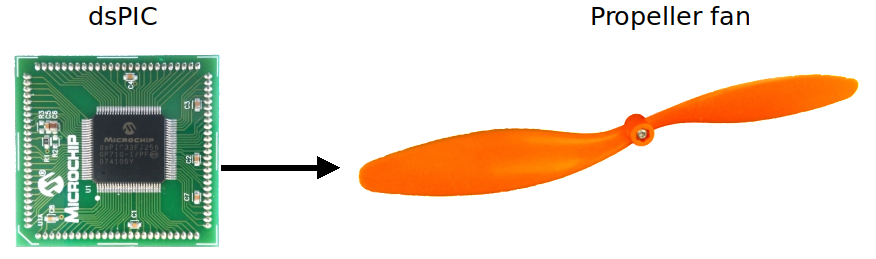
\includegraphics[width=0.8\textwidth]{alim-helice}
\caption{Contrôle de l'hélice par le dsPIC33.}
\label{fig:helice}
\end{figure}

Pour ce faire, vous allez devoir utiliser un module nommé \textit{Output Compare -- PWM}, décrit dans l’annexe de programmation du dsPIC.

Pour rappel, le principe de la génération d’ondes carrées peut être décrit comme un timer à deux seuils~:
\begin{itemize}
	\item Au lancement du timer, la borne de sortie \texttt{OCx} est à ‘1’.
	\item Lorsque le registre de comptage du timer atteint un premier seuil, nommé \texttt{OCxRS}, la sortie bascule à ‘0’.
	Le timer continue à s’incrémenter.
	\item Lorsque le registre de comptage atteint la valeur de période \texttt{PRx} , le timer retourne à zéro, et la sortie retourne à ‘1’.
\end{itemize}

En jouant sur la valeur des deux seuils, il est possible de générer n’importe quelle onde carrée.

Mode opératoire~:
\begin{itemize}
	\item Lisez la section du guide de programmation concernant le générateur PWM.
	\item Écrivez une routine permettant de générer sur une des bornes \texttt{OCx} une onde rectangulaire d’une période de 100~$\mu s$ et un rapport cyclique de 40~\%.
	Vérifiez ces valeurs à l’oscilloscope.
	\item Modifiez votre programme pour que cette routine se présente sous la forme d’une fonction permettant de facilement modifier le rapport cyclique sans modifier la période du signal.
	\item Connectez les bornes d’alimentation de l’hélice au 0V-5V du protoboard, et reliez l’entrée In1 ou In2 de l’hélice à votre sortie PWM.
	N’oubliez pas de relier les masses.
	\item Vérifiez que l’hélice tourne bien à vitesse variable.
\end{itemize}






%  #######     #####    ##      ##  ##     ##  #########  ########   ##########  ########    #######    #######   #########  ##     ##  ########   
% ##     ##  ##     ##  ###     ##  ##     ##  ##         ##     ##      ##         ##      ##     ##  ##     ##  ##         ##     ##  ##     ##  
% ##         ##     ##  ## ##   ##  ##     ##  ##         ##     ##      ##         ##      ##         ##         ##         ##     ##  ##     ##  
% ##         ##     ##  ##  ##  ##  ##     ##  ######     ########       ##         ##       #######    #######   ######     ##     ##  ########   
% ##         ##     ##  ##   ## ##   ##   ##   ##         ##   ##        ##         ##             ##         ##  ##         ##     ##  ##   ##    
% ##     ##  ##     ##  ##     ###    ## ##    ##         ##    ##       ##         ##      ##     ##  ##     ##  ##         ##     ##  ##    ##   
%  #######     #####    ##      ##     ###     #########  ##     ##      ##      ########    #######    #######   #########   #######   ##     ##  

\section{Utilisation en tant que convertisseur numérique-analogique}
La modulation PWM peut être appliquée à la conversion numérique-analogique.
% Le principe de ce convertisseur est présenté sur la figure suivante.

En éliminant les composantes hautes fréquences à l'aide d'un condensateur de découplage, on ne garde que la valeur moyenne du signal, à savoir $D(t) \cdot 3.3V$ , où $D(t)$ est l’évolution du rapport cyclique dans le temps\footnote{Une variante de ce principe, connue sous le nom de modulation Delta (ou Sigma Delta), est utilisée dans des convertisseurs analogique-numérique à haute résolution et basse fréquence, ainsi que dans le domaine de l’audio.}.

\begin{itemize}
	\item À l’aide d’un oscilloscope, analysez le spectre du signal PWM.
	\item Sur ce spectre, repérez l’effet de la modulation.
	\item Comment dimensionner le filtre RC afin d’éliminer la commutation~?
	\item Déduisez-en les limites de ce principe~: peut-on convertir n’importe quel signal~?
\end{itemize}


\end{document}
